Os avanços em algoritmos de controle têm permitido manobras autônomas mais sofisticadas, com menor intervenção humana e maior resiliência a falhas.

\subsection{Algoritmos baseados em IA}

A técnica de Machine Learning (ML) e Neural Network (NN) são usados para prever dinâmicas orbitais, identificar alvos e planejar trajetórias otimizadas em tempo real.

\subsubsection{Machine Learning}

Uma das utilidades da utilização do ML é a navegação autônoma de robôs móveis envolve o movimento eficiente de um agente artificial em direção a um destino, evitando colisões e lidando com incertezas ambientais. Essa área de pesquisa tem sido abordada ao longo das décadas por meio de métodos tradicionais, que combinam um planejamento global de trajetória com controle local de movimento. No entanto, esses métodos apresentam dificuldades ao lidar com ambientes altamente dinâmicos e não estruturados, onde as regras pré-definidas podem não ser suficientes para garantir uma navegação segura e eficiente \cite{xiao2022}.

Ainda conforme \cite{xiao2022} explica, com o crescimento da pesquisa em aprendizado de máquina, novas estratégias foram desenvolvidas para aprimorar a navegação autônoma, utilizando técnicas de aprendizado de dados em contraste com os métodos baseados em modelos simbólicos. As abordagens mais recentes incluem redes neurais profundas para aprendizado ponta a ponta, permitindo que robôs aprendam diretamente a relação entre percepção e ação sem a necessidade de um modelo explícito do ambiente, possibilitando que os sistemas se adaptem a diferentes cenários e melhorem sua capacidade de navegação em condições adversas. O lado negativo é que essas abordagens exigem grandes quantidades de dados e geralmente carecem de interpretabilidade, dificultando a compreensão e correção de erros que possam surgir durante a operação.

Outra utilização do ML é por conta da crescente proliferação de tecnologias espaciais e que tem gerado um aumento significativo na quantidade de detritos orbitais. Tais fragmentos, vindos de espaçonaves desativadas ou partes de satélites, representam um risco à navegação e à operação segura de veículos espaciais. Uma simples colisão com esses detritos pode resultar em danos estruturais e comprometer missões espaciais por completo, tornando a detecção e categorização dessas ameaças um aspecto essencial para a segurança orbital. A avaliação da densidade e do impacto potencial dos detritos tem sido um desafio constante, especialmente na órbita terrestre baixa (LEO), onde a concentração de objetos é elevada \cite{sri2024}.

A utilização de aprendizado de máquina para classificar e prever a periculosidade dos detritos orbitais tem sido explorada como alternativa aos métodos tradicionais baseados exclusivamente em modelos físicos. Esse método permite analisar grandes volumes de dados obtidos por sensores e sistemas de monitoramento espacial, fornecendo estimativas da ameaça representada por cada detrito com base em sua energia cinética e trajetória. Os métodos supervisionados de aprendizado têm sido empregados para identificar padrões nos dados e categorizar os detritos em diferentes níveis de risco, como baixo, médio e fatal. Essa classificação possibilita a criação de estratégias mais eficazes para mitigação de riscos, incluindo recomendações sobre o uso de revestimentos protetores em espaçonaves e o desenvolvimento de certificações de segurança para veículos espaciais \cite{sri2024}.

Ainda conforme \cite{sri2024}, o programa de detritos orbitais da NASA tem sido um dos principais referenciais para esse tipo de pesquisa, combinando análises físicas com modelagem matemática para prever a distribuição e os impactos dos detritos. O cruzamento dessas informações com técnicas de aprendizado de máquina contribui para a identificação precisa da localização dos fragmentos e para a avaliação da probabilidade de colisões. Dessa forma, a integração entre métodos computacionais e físicos tem se mostrado uma abordagem relevante para aprimorar a segurança no ambiente espacial e possibilitar um planejamento mais eficiente para futuras missões.

\subsubsection{Neural Network}

Segundo \cite{ke2018}, os modelos de redes neurais profundas (DNNs) têm sido amplamente empregados em diversas aplicações, como visão computacional, processamento de linguagem natural e tradução automática, porém, a execução desses modelos em plataformas computacionais convencionais, baseadas em CPUs, pode ser ineficiente devido à alta demanda por processamento paralelo e ao grande consumo de memória. Para lidar com essas limitações, diversas arquiteturas especializadas foram desenvolvidas, incluindo unidades de processamento gráfico (GPUs), matrizes de portas programáveis em campo (FPGAs) e circuitos integrados específicos para aplicações (ASICs). Essas soluções permitem explorar o paralelismo inerente aos modelos de DNNs e otimizar a execução de suas operações.

Ainda como explica \cite{ke2018}, a crescente complexidade das redes neurais e a diversidade de suas arquiteturas impõem desafios para o projeto de aceleradores eficientes. Cada rede possui características distintas que influenciam a eficiência da implementação em hardware, tornando inviável uma abordagem única que atenda a todas as configurações possíveis. Nesse contexto, abordagens de exploração de espaço de projeto (DSE) têm sido adotadas para avaliar diferentes pontos de design e estimar seu impacto no desempenho, consumo de energia e área ocupada pelo circuito. Ferramentas como o NNest foram desenvolvidas para facilitar essa análise, permitindo a modelagem de arquiteturas aceleradoras e a comparação de diferentes estratégias de movimentação de dados e ajuste de camadas.

Além da escolha da arquitetura do acelerador, outros fatores afetam a eficiência da execução das DNNs. As estratégias de reutilização de pesos e somas parciais podem reduzir a quantidade de operações redundantes, otimizando o uso dos recursos computacionais. Métodos de quantização, como redes neurais binárias (BNNs), também vêm sendo explorados para diminuir o consumo de energia e reduzir a complexidade computacional. Essas abordagens permitem equilibrar a relação entre precisão do modelo e eficiência computacional, tornando viável a implementação de DNNs em dispositivos embarcados com restrições de potência e área.

A utilização de DNNs continua a crescer, impulsionando a necessidade de arquiteturas especializadas que ofereçam alto desempenho e baixo consumo de energia. O desenvolvimento de novas técnicas de exploração de espaço de projeto e a integração de estratégias de otimização são fundamentais para garantir que essas redes possam ser aplicadas de forma eficiente em diferentes cenários.

A seguir serão expostos exemplos de capacidades autônomas.

\subsection{Boeing Starliner}

A espaçonave CST-100 Starliner da Boeing possui capacidades autônomas projetadas para garantir operações seguras e eficientes em missões espaciais. Abaixo, são detalhados cinco aspectos principais dessas funcionalidades.

\begin{figure}[H]
    \centering
    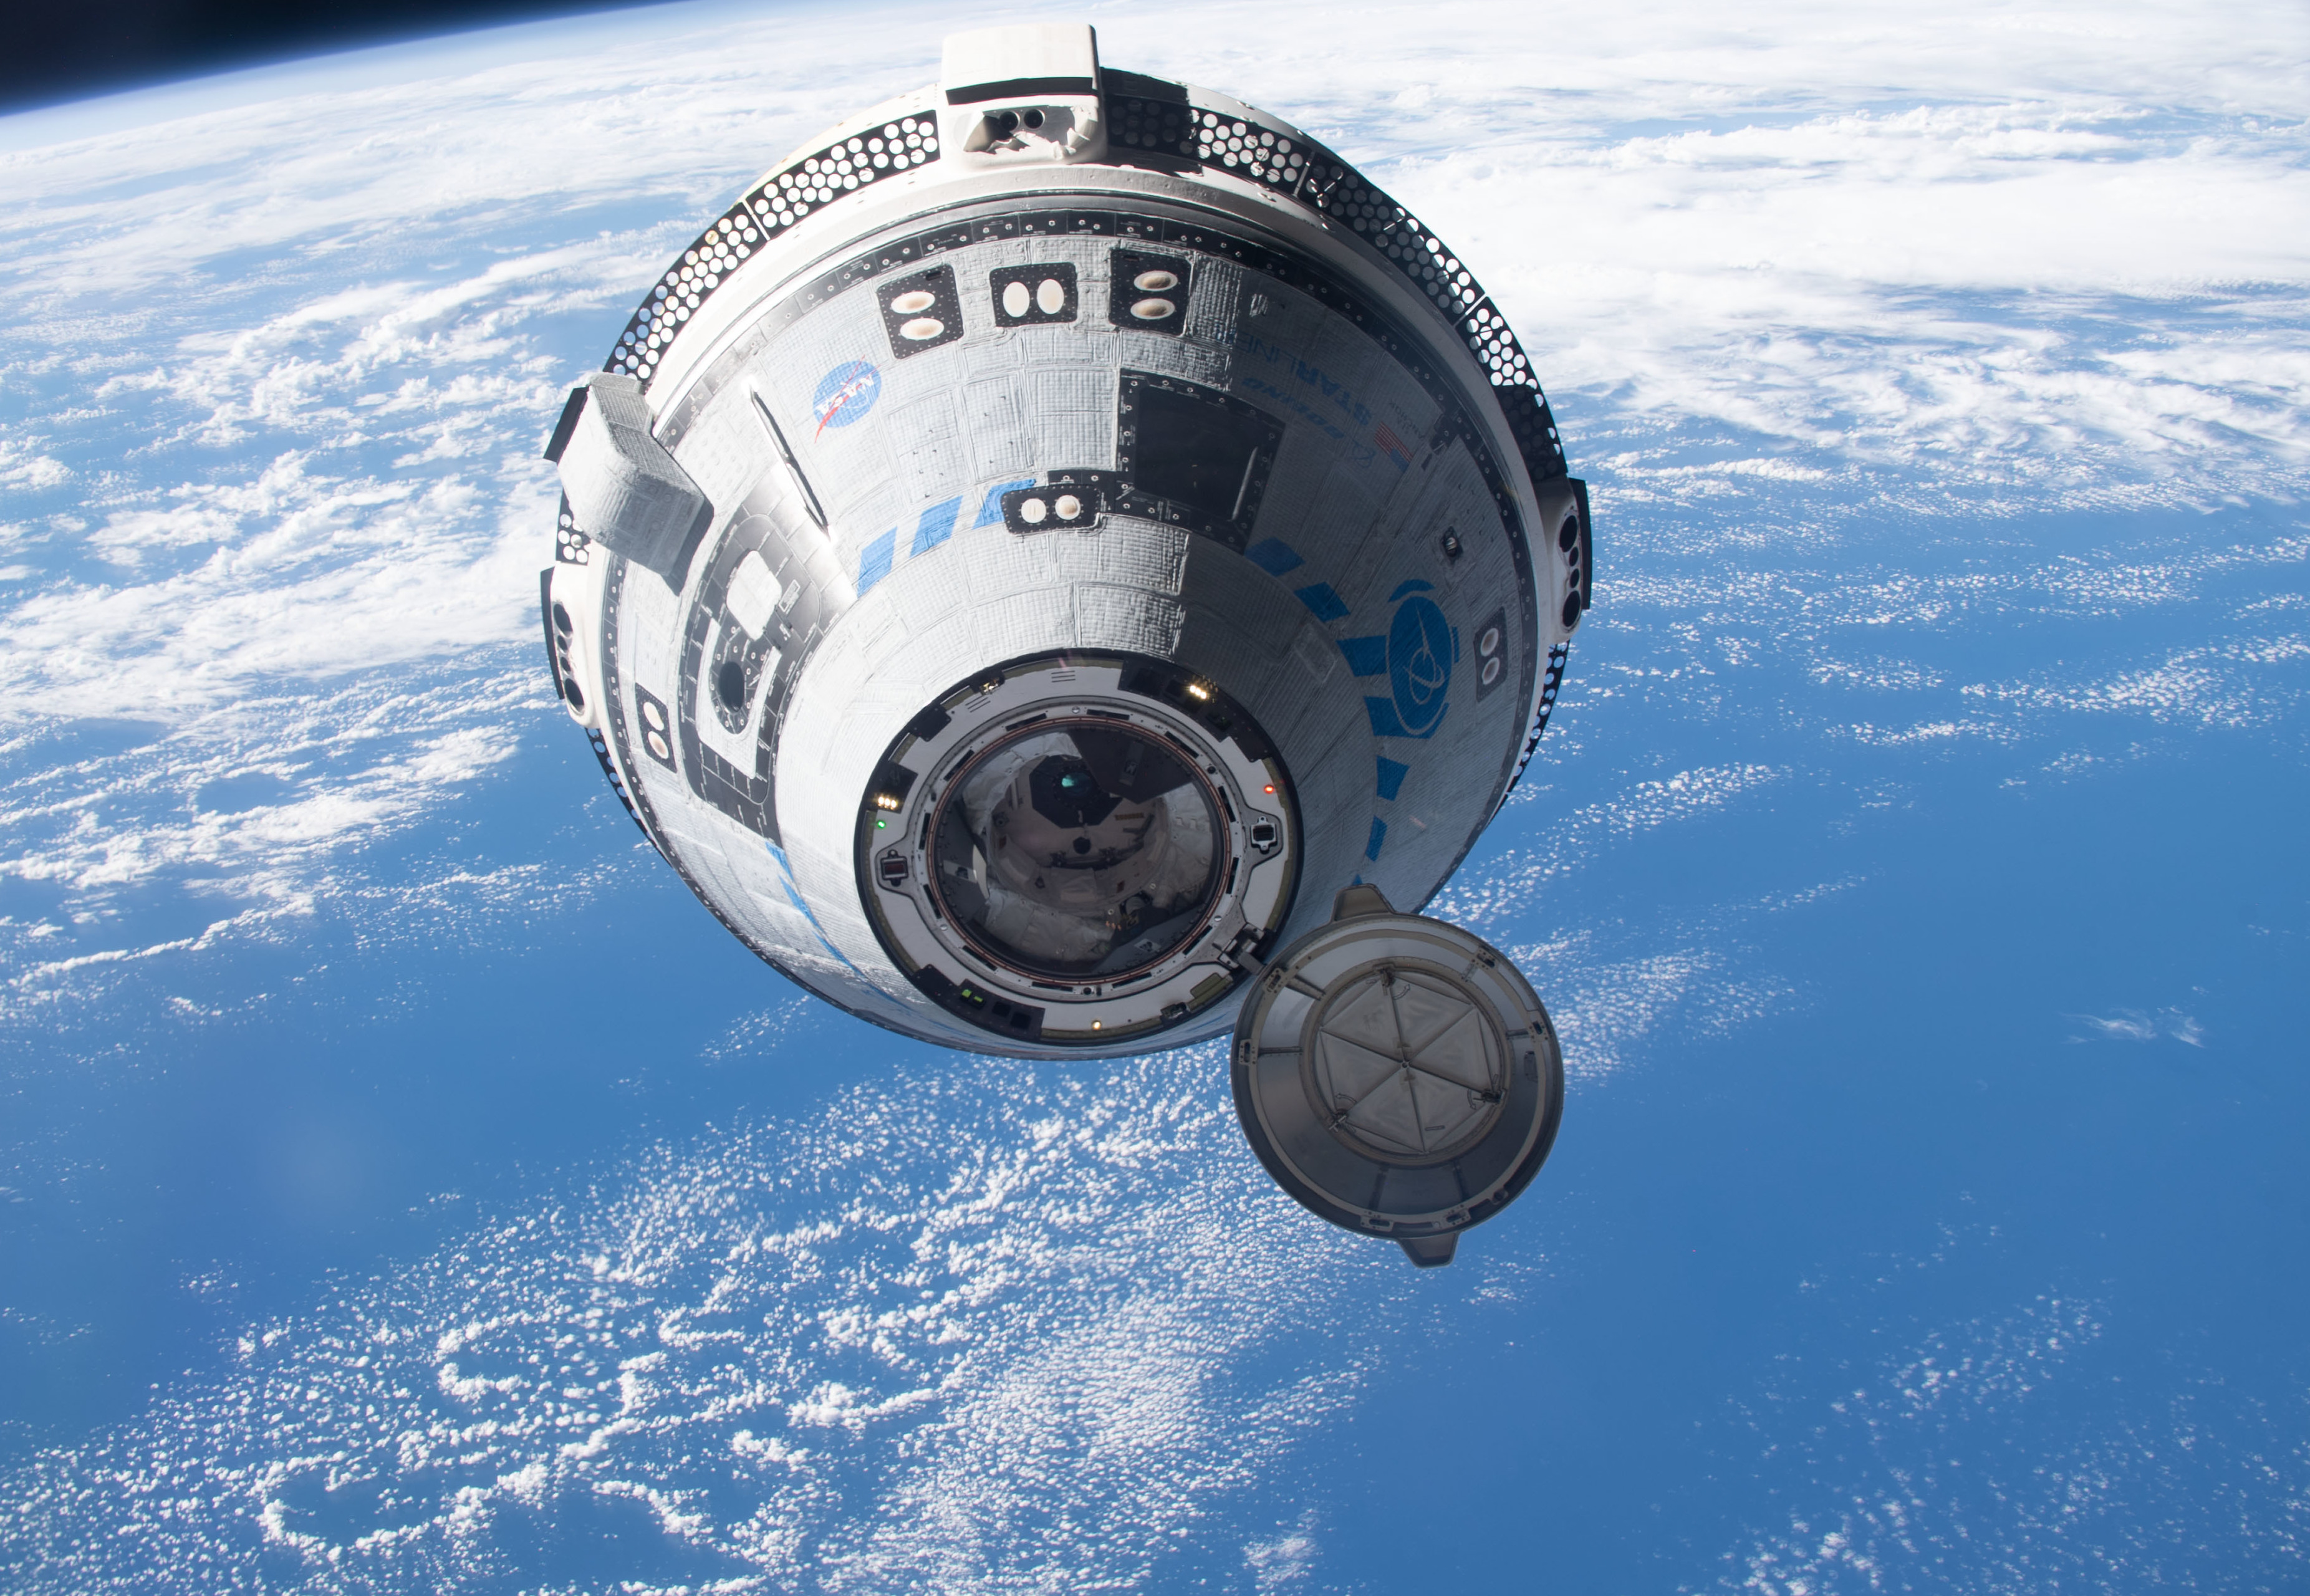
\includegraphics[width=0.75\linewidth]{RevDaLiteratura/Imagens/Boeing Starliner.jpg}
    \caption{Espaçonave Starliner da fabricante Boeing. Fonte: Boeing.}
    \label{fig:BoeingStarliner}
\end{figure}

\subsubsection{Navegação e Correção de Trajetória Autônomas}
A espaçonave Starliner pode realizar navegação de forma precisa com ajustes de curso de forma a não depender de humanos, sendo totalmente independente. Também é capaz de detectar e corrigir desvios ou erros em sua trajetória durante o voo, assegurando que cumpra o trajeto planejado \cite{boeing2024}.

\subsubsection{Acoplamento Automatizado com a ISS}
Por ser equipado com sistemas avançados de sensores e software, a espaçonave pode realizar manobras de rendezvous and docking junto à ISS sem intervenção humana, essa funcionalidade reduz a carga de trabalho dos astronautas e o risco de erros durante essas operações críticas \cite{boeing2024}.

\subsubsection{Capacidade de Autodiagnóstico e Recuperação}
A nave espacial está equipada com sistemas que monitoram constantemente seu próprio funcionamento e são capazes de detectar anomalias ou falhas. Em várias situações o Starliner pode realizar procedimentos de recuperação de forma automática para resolver questões identificadas e melhorar a resistência da missão \cite{boeing2024}.

\subsubsection{Operação com e sem Tripulação}
Embora tenha capacidade para transportar até setes passageiros no Starliner é possível executar missões autônomas sem tripulação presente. Essas possibilidades de design permitem que o veículo espacial seja empregado em outras funções como o transporte de carga ou testes de sistemas sem depender da intervenção humana \cite{boeing2024}.

\subsubsection{Interface de Controle Manual para Situações de Contingência}
Apesar de suas capacidades autônomas avançadas, o Starliner está equipado com interfaces que permitem aos astronautas assumir o controle manual da espaçonave quando necessário. Isso garante que, em situações imprevistas ou de emergência, a tripulação possa intervir e conduzir a espaçonave de forma segura \cite{boeing2024}.




